% -------------------------------------------------------------------------
%  MusicFormats Library
%  Copyright (C) Jacques Menu 2016-2023

%  This Source Code Form is subject to the terms of the Mozilla Public
%  License, v. 2.0. If a copy of the MPL was not distributed with this
%  file, you can obtain one at http://mozilla.org/MPL/2.0/.

%  https://github.com/jacques-menu/musicformats
% -------------------------------------------------------------------------

% !TEX root = mfuserguide.tex

% -------------------------------------------------------------------------
\chapter{Library components}\label{Library components}
% -------------------------------------------------------------------------

\mf\ uses the following terminology for its components:
\begin{itemize}
\item a \MainIt{format} is a description of music scores in textual of binary form, used in the field of music score applications, thus outside of the library;

\item a \MainIt{representation} in an internal data structure describing a music score. As of this writing, the supported representations are:
\begin{itemize}
\item \mxsrRepr\ (\mxml\ Score Representation);
\item \msrRepr\ (Music Score Representation);
\item \lpsrRepr\ (\lily\ Score Representation);
\item \bsrRepr\ (\braille\ Score Representation).
\end{itemize}

There is another, non-musical, \Main{representation} in \mf: \oahRepr\ contains a description of the options and help provided by the library and its 'musical' components.

\item the formats known to \mf\ can be seen as external representations of music scores, while representations are internal to the library;

\item a \MainIt{pass} performs a unitary conversion between a format and/or a representation to another such, as a \MainIt{single step}. This term comes from the compiler writing field: it means that the whole music score description is traversed to produce another description;

\item a \MainIt{converter} is a sequence of two or more passes. Each one converts a representation, either external or internal, into another that is used by the next pass in a pipeline way, at the higher level. \\
Such converters are thus said to be \MainIt{multi-pass}.

The first converter, provided by the \libmusicxml\ library, was {\tt xml2guido}.

Other converters provided by \mf\ were added later by this author, currently: \xmlToLy\, \xmlToBrl\, \xmlToXml\ and \xmlToGuido.

For example:
\begin{lstlisting}[language=Terminal]
jacquesmenu@macmini > xml2xml -about
What xml2xml does:

    This multi-pass converter basically performs 6 passes:
        Pass 1:  reads the contents of MusicXMLFile or stdin ('-')
                 and converts it to a MusicXML tree;
        Pass 2a: converts that MusicXML tree into
                 a first Music Score Representation (MSR) skeleton;
        Pass 2b: populates the MSR skeleton from the MusicXML tree
                 to get a full MSR;
        Pass 3:  converts the first MSR into a second MSR, to apply options;
        Pass 4:  converts the second MSR into a second MusicXML tree;
        Pass 5:  converts the second MusicXML tree to MusicXML code
                 and writes it to standard output.

    Other passes are performed according to the options, such as
    displaying views of the internal data or printing a summary of the score.

    The activity log and warning/error messages go to standard error.
\end{lstlisting}

\item a \MainIt{generator} is a multi-pass converter that creates the first represention of a score in the sequence \MainIt{ex-nihilo}, without reading any input file. The ones provided by \mf\ are \code{Mikrokosmos3Wandering} and \code{LilyPondIssue34}:
\begin{lstlisting}[language=Terminal]
jacquesmenu@macmini > Mikrokosmos3Wandering -musicxml -about
What Mikrokosmos3Wandering does:

    This multi-pass generator creates a textual representation
    of Zoltán Kodály's Mikrokosmos III Wandering score.
    It basically performs 4 passes when generating MusicXML output:

        Pass 1:  generate a first MSR for the Mikrokosmos III Wandering score
        Pass 2:  converts the first MSR a second MSR, to apply options;
        Pass 3:  converts the second MSR into an MusicXML tree;
        Pass 4:  converts the MusicXML tree to MusicXML code
                 and writes it to standard output.

    Other passes are performed according to the options, such as
    displaying views of the internal data or printing a summary of the score.

    The activity log and warning/error messages go to standard error.
\end{lstlisting}


\item \mf\ also provides various examples and services to create and manipulate music scores.%%%JMI
\end{itemize}

At the \CLI\ level, only the \converter s, \generator s and \oahRepr\ are available to the user. The other components are used behind the scenes by the latter.

The \mf\ \API s, on the other hand, give full access to all the components, more about this in Part~V. %%%JMI


% -------------------------------------------------------------------------
\section{Formats}\label{Formats}
% -------------------------------------------------------------------------

The formats supported by \mf\ are:
%\begin{adjustwidth}{-0.5cm}{-0.5cm}
\begin{center}
\small
\def \contentsWidth{0.6\textwidth}
\def \arraystretch{1.3}
%
\begin{longtable}[t]{lp{\contentsWidth}}
{Format} & {Description} \tabularnewline[0.5ex]
\hline\\[-3.0ex]
%
\mxml\ & a text containg markups such as \musicXmlMarkup{part-list}, \musicXmlMarkup{time} and \musicXmlMarkup{note};
\tabularnewline

\guido\ & a text containg markups such as {\tt $\backslash$barFormat}, {\tt $\backslash$tempo} and {\tt $\backslash$crescEnd};
\tabularnewline

\lily\ & a text containg commands such as {\tt $\backslash$header}, {\tt $\backslash$override} and {\tt $\backslash$transpose};
\tabularnewline

Jianpu \lily\ & a text containg \lily\ commands and the use of \lilyJianpu\ (\url {https://github.com/nybbs2003/lilypond-Jianpu/jianpu10a.ly}) to obtain a Jianpu (numbered) score instead of the default western notation.

\lilyJianpu\ should be accessible to LilyPond for it to produce the score. This file is provided in \fileName{lilypondstuff/jianpu};
\tabularnewline

\braille\ & a text containg 6-dot cells, as described in \url {http://www.brailleauthority.org/music/Music_Braille_Code_2015.pdf};
\tabularnewline

\msdlLang\ & a text describing a score in the \msdlLang\ language.
\tabularnewline

%\midi\ & binary data containg markups such as \musicXmlMarkup{part-list}, \musicXmlMarkup{time} and \musicXmlMarkup{note};
%\tabularnewline

\end{longtable}
\end{center}

% -------------------------------------------------------------------------
\section{Representations}\label{Representations}
% -------------------------------------------------------------------------

The representations used by \mf\ are:
%\begin{adjustwidth}{-0.5cm}{-0.5cm}
\begin{center}
\small
\def \contentsWidth{0.6\textwidth}
\def \arraystretch{1.3}
%
\begin{longtable}[t]{lp{\contentsWidth}}
{Representation} & {Description} \tabularnewline[0.5ex]
\hline\\[-3.0ex]
%
MSR & Music Score Representation, in terms of part groups, parts, staves, voices, notes, etc. This is the heart of the multi-format converters provided by \mf;
\tabularnewline

\mxsrRepr & a tree representing the \mxml\ markups such as \musicXmlMarkup{part-list}, \musicXmlMarkup{time} and \musicXmlMarkup{note};
\tabularnewline

LPSR & LilyPond Score Representation, i.e. MSR plus LilyPond-specific items such as {\tt $\backslash$score} blocks;
\tabularnewline

BSR & Braille Score Representation, with pages, lines and 6-dots cells;
\tabularnewline

MDSR & MIDI Score Representation, to be designed.
\tabularnewline

%\texttt{RandomMusic} & generates an \mxsrRepr\ representation containing random music and writes it as \mxml
%\tabularnewline
%
%services & a set of other demo programs such as {\tt countnotes}, {\tt xmltranspose} and {\tt partsummary}
%\tabularnewline
%
%\texttt{toBeWritten} & should generate an MSR containing some music and write it as \mxml, \lily and \braille
%\tabularnewline

\end{longtable}
\end{center}


% -------------------------------------------------------------------------
\section{Passes}\label{Passes}
% -------------------------------------------------------------------------

In the picture, the arrows show the available passes. They are:
%\begin{adjustwidth}{-0.5cm}{-0.5cm}
\begin{center}
\small
\def \contentsWidth{0.7\textwidth}
\def \arraystretch{1.3}
%
\begin{longtable}[t]{clp{\contentsWidth}}
{Arrow} & {Pass name} & {Description} \tabularnewline[0.5ex]
\hline\\[-3.0ex]
%
\texttt{1} & mxml2mxsr & reads \mxml\ data from a file or from \standardInput\ is '-' is supplied as the file name, and creates an \mxsrRepr\ representation containg the same data;
\tabularnewline

\texttt{2} & mxsr2mxml & converts an \mxsrRepr\ representation into \mxml\ data. This is a mere 'print()' operation;
\tabularnewline

\texttt{3} & mxsr2guido & converts an \mxsrRepr\ representation into Guido text code, and writes it to \standardOutput;
\tabularnewline

\texttt{4} & mxsr2msr & converts an \mxsrRepr\ representation into and \msrRepr\ representation. \mxml\ represents how a score is to be drawn, while MSR represents the musical contents with great detail. This pass actually consists in two sub-passes: the first one builds an MSR skeleton containing empty voices and stanzas, and the second one the fills this with all the rest;
\tabularnewline

\texttt{5} & mxsr2lpsr & converts an \msrRepr\ representation into an \lpsrRepr\ representation, which contains an MSR component build from the original MSR (pass 5). The BSR contains \lily-specific formats such as {\tt $\backslash$layout}, {\tt $\backslash$paper}, and {\tt $\backslash$score} blocks;
\tabularnewline

\texttt{6} & lpsr2msr & converts an \lpsrRepr\ representation into an \msrRepr\ representation. There is nothing to do, since the former contains the latter as a component;
\tabularnewline

\texttt{7} & lpsr2lilypond & converts an \lpsrRepr\ representation into LilyPond\ text code, and writes it to \standardOutput;
\tabularnewline

\texttt{7'} & lpsr2lilypond & converts an \lpsrRepr\ representation into LilyPond\ text code using \lilyJianpu, and writes it to \standardOutput. This pass is run with {\tt xml2ly -jianpu};
\tabularnewline

\texttt{8} & msr2bsr & converts an \msrRepr\ representation into a \bsrRepr representation, which contains an MSR component built from the original MSR. The BSR contains \braille-specific formats such as pages, lines and 6-dot cells. The lines and pages are virtual, i.e. not limited in length. This the pass where skip (invisible) notes are added wherever needed to avoid the \lily\ \#34 issue;
\tabularnewline

\texttt{9} & bsr2msr & converts a \bsrRepr representation into an \msrRepr\ representation. There is nothing to do, since the former contains the latter as a component;
\tabularnewline

\texttt{10} & bsr2bsr & converts a \bsrRepr representation into another one, to adapt the number of cells per line and lines per page from virtual to physical. Currently, the result is a mere clone;
\tabularnewline

\texttt{11} & bsr2braille & converts a \bsrRepr representation into \braille\ text, and writes it to \standardOutput;
\tabularnewline

\texttt{12} & msr2mxsr & converts an \msrRepr\ representation into an \mxsrRepr\ representation;
\tabularnewline

\texttt{13} & msr2msr & converts an \msrRepr\ representation into another one, built from scratch. This allows the new representation to be different than the original one, for example to change the score after is has been scanned and exported as \mxml\ data, or apply options;
\tabularnewline

\texttt{14} & msdl2msr & converts an \msdlLang\ score description into an \msrRepr\ representation.
\tabularnewline

\end{longtable}
\end{center}


% -------------------------------------------------------------------------
\section{Generators}\label{Generators}
% -------------------------------------------------------------------------

The ones generators by \libmusicxml\ create an \mxsrRepr\ representation and output it as \mxml\ text:
\begin{itemize}
\item \libmusicxmlSamples{RandomMusic.cpp} \\
generates an \mxsrRepr\ representation containing random music, and writes it as \mxml\ to \standardOutput;

\item \libmusicxmlSamples{RandomChords.cpp}:\\
generates an \mxsrRepr\ representation containing random two-note chords, and writes it as \mxml\ to \standardOutput;
\end{itemize}

\mf\ supplies its own generators to demonstrate the use of its \API s:
%\begin{itemize}JMI
%\item create a \mf\ representation ex-nihilo;
%
%\item convert it to some output format produces on \standardOutput, depending on which of the \optionName{lilypond}, \optionName{braille}, \optionName{musicxml} and \optionName{guido} options is used. Exactly one of those should be present.
%\end{itemize}
These generators are:
\begin{itemize}
\item \clisamples{MusicAndHarmonies.cpp}: \\
builds an \mxsrRepr\ representation containing notes and harmonies, and writes it as \mxml\ to \standardOutput:
\begin{lstlisting}[language=MusicXML]
jacquesmenu@macmini > MusicAndHarmonies | more
<?xml version="1.0" encoding="UTF-8" standalone="no"?>
<!DOCTYPE score-partwise PUBLIC "-//Recordare//DTD MusicXML 3.1 Partwise//EN"
                        "http://www.musicxml.org/dtds/partwise.dtd">
<score-partwise>
    <movement-title>Random Music</movement-title>
    <identification>
        <creator type="Composer">Georg Chance</creator>
        <encoding>
            <software>MusicFormats Library's MusicAndHarmonies generator</software>
        </encoding>
    </identification>
    <part-list>
        <score-part id="P1">
            <part-name>Part name</part-name>
            <score-instrument id="I1">
                <instrument-name>Any instr.</instrument-name>
            </score-instrument>
        </score-part>
    </part-list>
    <part id="P1">
        <measure number="1">
            <attributes>
                <divisions>4</divisions>
                <time>
                    <beats>4</beats>
                    <beat-type>4</beat-type>
                </time>
                <clef>
                    <sign>G</sign>
                    <line>2</line>
                </clef>
            </attributes>
            <harmony>
                <root>
                    <root-step>C</root-step>
                </root>
                <kind text="FOO">major</kind>
                <staff>1</staff>
            </harmony>
            <note>
                <pitch>
                    <step>F</step>
                    <octave>5</octave>
                </pitch>
                <duration>4</duration>
                <type>quarter</type>
            </note>

	<!-- ... ... ... -->
\end{lstlisting}


\item \clisamples{Mikrokosmos3Wandering.cpp}: \\
creates an \msrRepr\ graph representing Bartok's Mikrokosmos III Wandering score, and then produces \lily, \braille, \mxml\ or \guido\ from it. The \lily\ output gives:\\
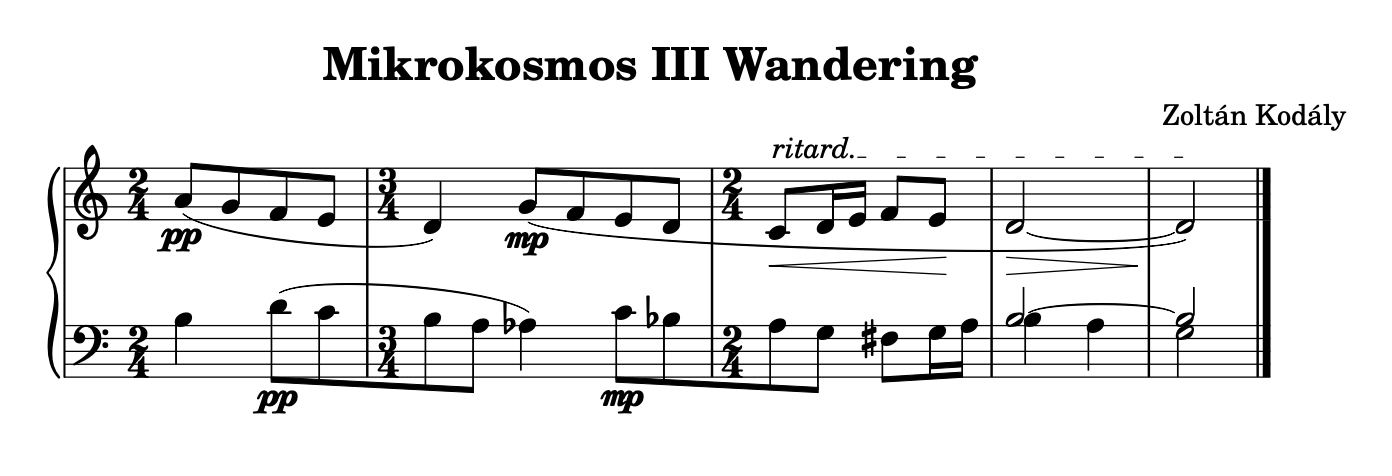
\includegraphics[scale=0.7]{../mfgraphics/Mikrokosmos_III_Wandering.png}

\item \clisamples{LilyPondIssue34.cpp}: \\
aims at creating an \lpsrRepr\ graph representing the score below, and then produces \lily, \braille, \mxml\ or \guido\ from it. Currently, the code is the same as that of \code{Mikrokosmos3Wandering}, though:\\
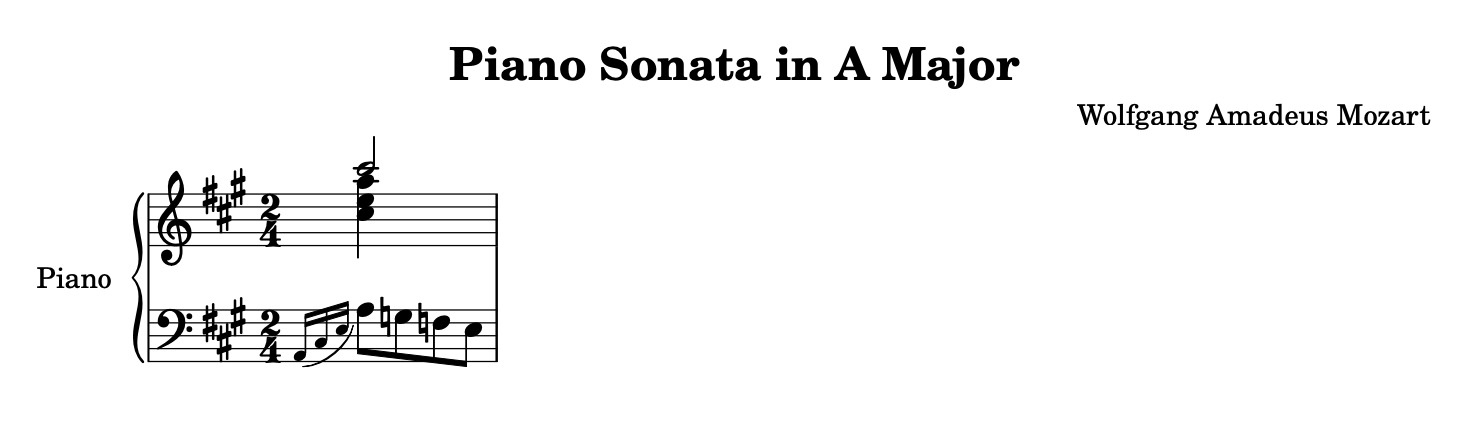
\includegraphics[scale=0.7]{../mfgraphics/LilyPondIssue34.png}
\end{itemize}


% -------------------------------------------------------------------------
\section{General use converters}\label{General use converters}
% -------------------------------------------------------------------------

The available \mxml\ converters available in \mf\ are:
%\begin{adjustwidth}{-0.5cm}{-0.5cm}
\begin{center}
\small
\def \contentsWidth{0.7\textwidth}
\def \arraystretch{1.3}
%
\begin{longtable}[t]{lp{\contentsWidth}}
{Converter} & {Description} \tabularnewline[0.5ex]
\hline\\[-3.0ex]
%

\xmlToGuido & supplied by \libmusicxml, converts \mxml\ data to Guido code, using passes:

\tab\ 1 $\Rightarrow$ 3
\tabularnewline


\xmlToLy & performs the 4 passes from \mxml\ to LilyPond\ to translate the former into the latter, using these passes:

\tab\ 1 $\Rightarrow$ 4 $\Rightarrow$ 13 $\Rightarrow$ 5 $\Rightarrow$ 7

The \optionName{jianpu} option is supplied to create Jianpu (numbered) scores, in which the notes are represented by numbers instead of graphics, using passes:

\tab\ 1 $\Rightarrow$ 4 $\Rightarrow$ 13 $\Rightarrow$ 5 $\Rightarrow$ 7'
\tabularnewline


\xmlToBrl & performs the 5 passes from \mxml\ to \braille\ to translate the former into the latter (draft);

\tab\ 1 $\Rightarrow$ 4 $\Rightarrow$ 13 $\Rightarrow$ 8 $\Rightarrow$ 10 $\Rightarrow$ 11
\tabularnewline


\xmlToXml & converts \mxml\ data to MSR and back in 5 passes. This is useful to modify \mxml\ data to suit the user's needs, such as fixing score scanning software limitations or to enhance the data:

\tab\ 1 $\Rightarrow$ 4 $\Rightarrow$ 13 $\Rightarrow$ 12 $\Rightarrow$ 2
\tabularnewline


\xmlToGmn & converts \mxml\ data to Guido code, using passes:

\tab\ 1 $\Rightarrow$ 4 $\Rightarrow$ 13 $\Rightarrow$ 12 $\Rightarrow$ 3
\tabularnewline

\end{longtable}
\end{center}

The passes used by the converters are shown by their \optionNameBoth{about}{a} option. For example:
\begin{lstlisting}[language=Terminal]
jacquesmenu@macmini > xml2xml -about
What xml2xml does:

    This multi-pass converter basically performs 6 passes:
        Pass 1:  reads the contents of MusicXMLFile or stdin ('-')
                 and converts it to a MusicXML tree;
        Pass 2a: converts that MusicXML tree into
                 a first Music Score Representation (MSR) skeleton;
        Pass 2b: populates the MSR skeleton from the MusicXML tree
                 to get a full MSR;
        Pass 3:  converts the first MSR into a second MSR, to apply options;
        Pass 4:  converts the second MSR into a second MusicXML tree;
        Pass 5:  converts the second MusicXML tree to MusicXML code
                 and writes it to standard output.

    Other passes are performed according to the options, such as
    displaying views of the internal data or printing a summary of the score.

    The activity log and warning/error messages go to standard error.
\end{lstlisting}

Since the generators may produce various output formats, one should be specified:
\begin{lstlisting}[language=Terminal]
jacquesmenu@macmini > Mikrokosmos3Wandering -about
What Mikrokosmos3Wandering does:

    This multi-pass generator creates a textual representation
    of Zoltán Kodály's Mikrokosmos III Wandering score.
    It performs various passes depending on the output generated,
    which should be specified a '-lilypond', '-braille', '-musicxml' or '-guido' option.

    Other passes are performed according to the options, such as
    displaying views of the internal data or printing a summary of the score.

    The activity log and warning/error messages go to standard error.
\end{lstlisting}

Adding \option{braille}, for example we get:
\begin{lstlisting}[language=Terminal]
jacquesmenu@macmini > Mikrokosmos3Wandering -braille -about
What Mikrokosmos3Wandering does:

    This multi-pass generator creates a textual representation
    of Zoltán Kodály's Mikrokosmos III Wandering score.
    It basically performs 4 passes when generating braille output:

        Pass 1:  generate a first MSR for the Mikrokosmos III Wandering score
        Pass 2:  converts the first MSR a second MSR, to apply options;
        Pass 3:  converts the second MSR into a
                 Braille Score Representation (BSR)
                 containing one Braille page per MusicXML page;
        Pass 4:  converts the BSRinto another BSR
                 with as many Braille pages as needed
                 to fit the line and page lengthes;
        Pass 5:  converts the BSR to Braille text
                 and writes it to standard output.)

    In this preliminary version, pass 3 merely clones the BSR it receives.

    Other passes are performed according to the options, such as
    displaying views of the internal data or printing a summary of the score.

    The activity log and warning/error messages go to standard error.
\end{lstlisting}


% -------------------------------------------------------------------------
\section{Specific converters}\label{Specific converters}
% -------------------------------------------------------------------------

\mf\ provides only one compiler in the usual software meaning, namely \msdlconverter.

\msdlLang\ (Music Score Description Language) is a language under evolution being created by this author. It is meant for use by musicians, i.e. non-programmers, to obtain scores from a rather high-level description.\\
\mf supplies {\tt msdl}, a compiler converting \msdlLang\ into \guido\, \lily, \braille or \mxml\ to \standardOutput, depending on the '{\tt -generated-code-kind}' option.

%\begin{adjustwidth}{-0.5cm}{-0.5cm}
\begin{center}
\small
\def \contentsWidth{0.7\textwidth}
\def \arraystretch{1.3}
%
\begin{longtable}[t]{lp{\contentsWidth}}
{Translator} & {Description} \tabularnewline[0.5ex]
\hline\\[-3.0ex]
%


\msdlconverter\ \optionName{lilypond} & performs the 4 passes from \mxml\ to LilyPond\ to translate the former into the latter, using these passes:

\tab\ 1 $\Rightarrow$ 4 $\Rightarrow$ 13 $\Rightarrow$ 5 $\Rightarrow$ 7

The \optionName{jianpu} option is supplied to create Jianpu (numbered) scores, in which the notes are represented by numbers instead of graphics, using passes:

\tab\ 1 $\Rightarrow$ 4 $\Rightarrow$ 13 $\Rightarrow$ 5 $\Rightarrow$ 7'
\tabularnewline


\msdlconverter\ \optionName{braille} & performs the 5 passes from \mxml\ to \braille\ to translate the former into the latter (draft);

\tab\ 1 $\Rightarrow$ 4 $\Rightarrow$ 13 $\Rightarrow$ 8 $\Rightarrow$ 10 $\Rightarrow$ 11
\tabularnewline



\msdlconverter\ \optionName{musicxml} & converts \mxml\ data to MSR and back. This is useful to modify the data to suit the user's needs, such as fixing score scanning software limitations or to enhance the data:

\tab\ 1 $\Rightarrow$ 4 $\Rightarrow$ 13 $\Rightarrow$ 12 $\Rightarrow$ 2
\tabularnewline



\msdlconverter\ \optionName{guido} & converts \mxml\ data to Guido code, using passes:

\tab\ 1 $\Rightarrow$ 4 $\Rightarrow$ 13 $\Rightarrow$ 12 $\Rightarrow$ 3
\tabularnewline

\end{longtable}
\end{center}


% -------------------------------------------------------------------------
\section{MusicFormats services}
% -------------------------------------------------------------------------

The \mf\ library provides \MainIt{services} to the user. As of this writing, they are:
\begin{itemize}
\item generators;
\item converters.
\end{itemize}

Other services may be provided in the future, such as music score analyzers.

This is why this documentation uses the term \MainIt{service} for the current \generator s and \converter s.


% -------------------------------------------------------------------------
\section{Other tools}
% -------------------------------------------------------------------------

\libmusicxml\ supplies a number of basic tools using its features:

\begin{itemize}
\item {\tt xmlread} converts \mxml\ data and displays the corresponding xmlElement tree;

\item {\tt countnotes} reads \mxml\ data and displays the number of notes it contains;

\item other programs such as {\tt xmltranspose} and {\tt partsummary} demonstrate the possibilities of the library, in particular those of the two-phase visitors pattern it uses.

\item {\tt xml2midi} reads \mxml\ data and outputs a midi version of it.
\end{itemize}

It is to be noted that:
\begin{itemize}
\item \lily\ provides \midiToLy\ to translate MIDI files to LilyPond\ code;
\item \lily\ can generate MIDI files from its input.
\end{itemize}


